% DRAFT sections for the FINAL report (due 9 Apr 2027): Results, Discussion, Conclusion.
% Not part of the interim report. Include with % DRAFT sections for the FINAL report (due 9 Apr 2027): Results, Discussion, Conclusion.
% Not part of the interim report. Include with % DRAFT sections for the FINAL report (due 9 Apr 2027): Results, Discussion, Conclusion.
% Not part of the interim report. Include with % DRAFT sections for the FINAL report (due 9 Apr 2027): Results, Discussion, Conclusion.
% Not part of the interim report. Include with \input{final_report_results_DRAFT} inside the final report's main.tex.
% Every number comes from ../analysis/results/results_tables.md (checked by ../analysis/check_results.py).
% The student must rewrite this in their own words (university AI-writing policy) and understand every sentence.
% Needs \usepackage{booktabs} for the tables and the figures in ../analysis/figures/.
% The word limit for the final report is not known yet: check the final-report template before keeping all of this.

\section{Results}\label{sec:results}

\subsection{Set-up}
Models were evaluated by rolling-origin testing on 146 weeks (7 January 2024 to 18 October 2026), with an expanding training window and a weekly re-fit. Hyper-parameters were re-tuned every 26 weeks using only the data available at that origin. Differences in mean absolute error (MAE) were tested with the Diebold--Mariano test \parencite{diebold1995} at the 5\% level, with the Holm correction across QEUH and GRI; RHC is exploratory and uncorrected. The primary comparisons, named before the tables were read, are M2 against M1 (H$_1$) and M2 against B2 (H$_2$) at QEUH and GRI, one week ahead; everything else is secondary or exploratory. The weather used in the main experiment is the observed (reanalysis) weather of the target week, so the main results show what weather can add when it is known (a nowcast); Section~\ref{sec:res-fw} uses real archived forecasts. Because M2 contains M1, the Diebold--Mariano asymptotics are approximate and borderline results are not decisive.

\subsection{Baselines and models, one week ahead}
\begin{table}[h!]
\centering\small
\begin{tabular}{lccc}
\hline
MAE (attendances per week) & QEUH & GRI & RHC \\
\hline
B1 seasonal naive & 84.6 & 79.8 & 105.6 \\
B2 last week & 70.6 & 68.1 & 96.8 \\
M1 GAM, no weather & 62.8 & 61.5 & 91.0 \\
M2 GAM with weather & 54.7 & 57.2 & 83.3 \\
M3 XGBoost, all features & 53.1 & 57.7 & 85.0 \\
M3a XGBoost, no weather & 56.7 & 60.2 & 86.7 \\
\hline
\end{tabular}
\caption{One-week-ahead errors on the 146 test weeks.}
\label{table:res-main}
\end{table}

\textbf{H$_2$ (beats the baselines, with observed weather).} M2 had a lower MAE than last week's attendance by 22.5\% at QEUH and 16.0\% at GRI (all Holm-adjusted $p<0.001$), and by 13.9\% at RHC. It also beat the seasonal baseline at every hospital.

\textbf{H$_1$ (weather adds value).} At QEUH, M2 reduced MAE by 12.9\% compared with the same model without weather (62.8 to 54.7; Holm-adjusted $p<0.001$). At GRI the reduction was 7.1\% (61.5 to 57.2) but the difference was not significant at the 5\% level ($p=0.054$), so the null hypothesis is not rejected there; with a Newey--West variance the same comparison gave $p=0.024$ and $0.015$ (3 and 8 lags), so GRI is best described as inconclusive. At RHC (exploratory) the difference was significant ($p=0.002$, uncorrected). About half of M2's improvement over last week at QEUH comes from the calendar and autoregressive terms: M1 alone has 11.1\% skill against last week, M2 has 22.5\%.

At one week ahead XGBoost did not improve on the GAM: M3 and M2 did not differ significantly (Holm $p=0.935$ at both adult hospitals). At two weeks ahead M3 was lower than M2 at QEUH (54.1 against 59.6) but not significantly so after correction (Holm $p=0.059$).

\begin{figure}[h!]
\centering
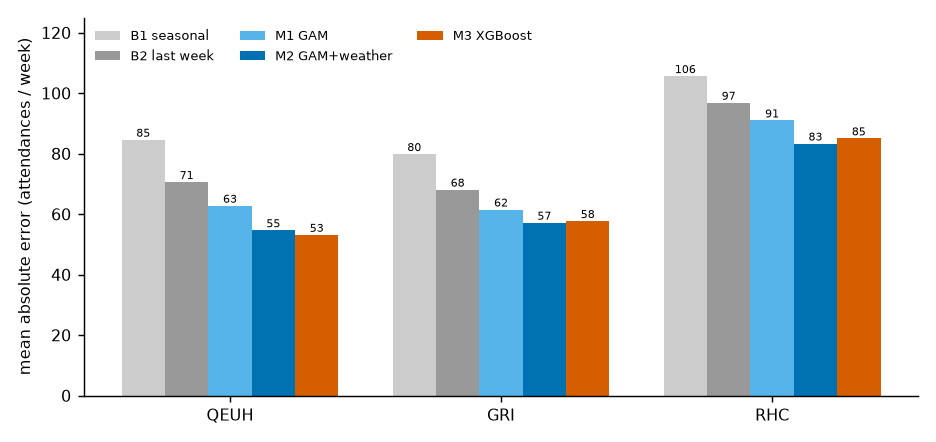
\includegraphics[width=0.9\textwidth]{../analysis/figures/fig_mae.png}
\caption{MAE by model and hospital, one week ahead.}
\end{figure}

\subsection{Which environmental factors matter}
Adding groups of weather variables to M1 one at a time showed that temperature carries the gain. Temperature alone gave MAE 54.9 (QEUH) and 57.7 (GRI), against 54.7 and 57.2 for all weather combined. Air quality alone (62.2 and 61.6) and humidity and rain alone (62.8 and 61.6) gave no improvement over M1 (all $p>0.4$ at the adult hospitals). A placebo model that was given the weather of the same week one year earlier lost the gain (QEUH 61.8, GRI 61.9), so the improvement is not a seasonal effect but depends on the temperature of the week itself.

The fitted GAM uses both this week's and last week's temperature, and the association is predictive, not causal. Moving only this week's temperature from the 5th to the 95th percentile (2.1 to 16.0\,$^\circ$C) with last week's temperature at its average was associated with about 150 more attendances at QEUH (8.1\% of the mean), 132 at GRI (8.0\%) and 153 at RHC (11.5\%). When last week's temperature moved with it, the association shrank to 38 at QEUH (2.0\%), 23 at GRI (1.4\%) and $-28$ at RHC. The signal is therefore mainly the week-to-week change in temperature: about 9.6 more attendances at QEUH and 9.8 at GRI for each degree a week is warmer than the previous one (about 0.5\% of weekly attendance). Weekly mean temperature in the test period stayed below 18\,$^\circ$C, so this says nothing about heatwaves.

\begin{figure}[h!]
\centering
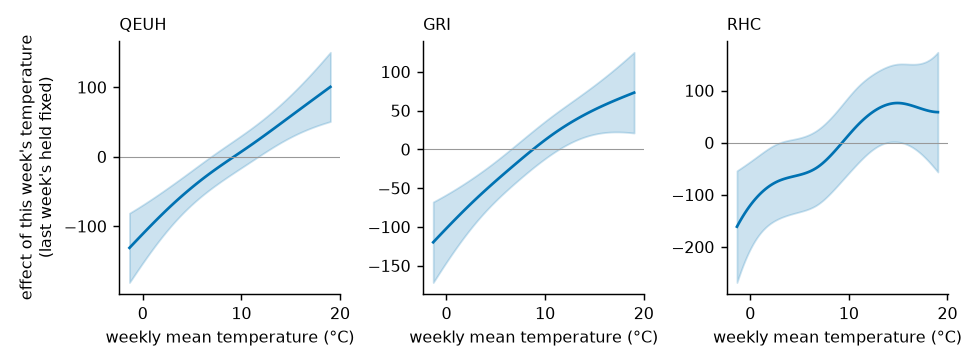
\includegraphics[width=0.9\textwidth]{../analysis/figures/fig_temperature_effect.png}
\caption{Association of this week's mean temperature with attendance (95\% band), with last week's temperature held fixed.}
\end{figure}

\subsection{Robustness}
Excluding flagged weeks from the training data did not change the one-week-ahead conclusions (QEUH: M2 52.3 against M1 60.6; GRI: 56.3 against 60.5; RHC: 77.7 against 86.8); the test weeks contain no flagged week. At two and four weeks ahead M2 beat M1 at QEUH (Holm $p=0.002$ at both horizons) but not at GRI or RHC, and the four-week result at QEUH is not significant when flagged weeks are excluded (Holm $p=0.236$). These longer horizons are not realistic forecasts, because the model sees the observed weather of a week that could not be known so far ahead; they are upper bounds.

\subsection{Real forecast weather}\label{sec:res-fw}
Archived ECMWF forecasts are available only from March 2024, so this experiment uses 135 of the 146 test weeks. Models trained on reanalysis weather were tested on the forecast issued the Sunday before each week (weekly mean-temperature error against reanalysis: RMSE 0.68\,$^\circ$C, bias $+0.30$\,$^\circ$C). At QEUH the gain was kept in full (MAE 54.4 against 62.4 for M1, Holm $p<0.001$). At GRI only part of it was kept: 59.9 against 62.9, not significant ($p=0.252$), and significantly worse than with observed weather (Holm $p=0.026$); its skill against last week was 13.2\%, below the 15\% target set in the proposal. The temperature-only model (M2t) was as good as M2 with forecast weather (54.3, 60.0 and 83.3 at QEUH, GRI and RHC), and is the model used in the prototype.

\subsection{Alerts}
A high-pressure week was defined as one above the 90th percentile of the previous 52 weeks. The first evaluation was for M2 with observed weather; the temperature-only model used in the prototype, real forecast weather and a ``medium'' tier (above the 75th percentile) were evaluated afterwards from the same forecasts (Section~5b of the results file). At QEUH, M2 raised 11 alerts for 21 high weeks, with precision 0.64 (95\% interval 0.35 to 0.85), recall 0.33 (0.17 to 0.55) and 0.12 false alarms per month; last-week persistence had recall 0.43 but precision 0.41 and 0.39 false alarms per month. At GRI, M2 had precision 0.55 and recall 0.44. At RHC (exploratory) M2 had precision 0.73 and recall 0.55 against 0.60 and 0.60 for persistence. At the two adult hospitals no model identified most high-pressure weeks, and the intervals are wide because there are few alerts. With the temperature-only model on real forecasts, the QEUH alert had precision 0.62 and recall 0.38 against a base rate of 15.6\%, with 0.16 false alarms per month, against 0.42 for last-week persistence at similar recall; at GRI the intervals overlapped with persistence, so no advantage was shown. The medium tier was only modestly informative (QEUH precision 0.60 against a base rate of 37.0\%) and the prototype keeps it as watch-only.

\section{Discussion}
The results support the central claim that weekly A\&E attendance in Glasgow can be forecast more accurately than by repeating last week, and that temperature explains part of that gain at the largest adult hospital. The pattern is consistent with the positive association between temperature and A\&E attendances reported for London \parencite{corcuerahotz2020}, although that study used daily data and a different method. It differs from the finding that temperature gave no better forecasts than calendar variables in S\~ao Paulo \parencite{marcilio2013}; the settings, the time scale (daily against weekly) and the three-month test window of that study are possible reasons, but this project cannot tell. The finding that a GAM matched XGBoost agrees with the observation that linear models are often as good as tree ensembles \parencite{vollmer2021}.

The gains are real but modest in absolute terms: about 8 attendances a week at QEUH on a weekly mean of about 1,850. The evidence for weather is strongest at QEUH, weaker at GRI (not significant under Holm correction, and partly lost with real forecasts), and exploratory at RHC. Evaluation choices matter: a rolling-origin test against a persistence baseline \parencite{garciacrespi2026} was used here, and the calendar and autoregressive terms accounted for about half of the improvement over last week, which a comparison with a seasonal baseline alone would have hidden.

\textbf{Limitations.} The test covers one city and 146 weeks; one weather grid cell stands for all three hospitals; the counts are all-cause and the data hold no infection information, so warm-week effects may partly reflect other seasonal factors. The result is predictive, not causal. The evaluation is not a real-time one: it assumes last week's attendance is known on the Sunday night, although the data are published with a delay, and it uses final, not first-release, figures. The model specifications were set before the experiments were run, to the author's knowledge, but the ablation, the placebo and the choice of the temperature-only model for the prototype came afterwards. Holm correction covers two hospitals per comparison, not the roughly 540 tests run, and the Diebold--Mariano test is approximate for nested models. Weather is reanalysis, not station data, and air quality is modelled. Hot-day thresholds were set from percentiles of pre-2024 temperatures, not from the GAM curves as planned in the interim report.

\section{Conclusion}
Weekly A\&E attendance at QEUH and GRI can be forecast better than by last week's value or the same week last year (reductions in MAE of 22.5\% and 16.0\% against last week). Temperature adds significant accuracy at QEUH (12.9\%) and inconclusively at GRI (7.1\%, $p=0.054$), mainly through the week-to-week change in temperature; air quality, humidity and rain add nothing. With real forecasts the gain holds at QEUH and weakens at GRI. The prototype turns the model into a one-week forecast with a risk class, an explanation of its drivers and a human approval step, but its alerts miss most high-pressure weeks at the adult hospitals and should be treated as a prompt for review. Future work includes infection data, station weather, school terms and local holidays, and testing across other Scottish boards.
 inside the final report's main.tex.
% Every number comes from ../analysis/results/results_tables.md (checked by ../analysis/check_results.py).
% The student must rewrite this in their own words (university AI-writing policy) and understand every sentence.
% Needs \usepackage{booktabs} for the tables and the figures in ../analysis/figures/.
% The word limit for the final report is not known yet: check the final-report template before keeping all of this.

\section{Results}\label{sec:results}

\subsection{Set-up}
Models were evaluated by rolling-origin testing on 146 weeks (7 January 2024 to 18 October 2026), with an expanding training window and a weekly re-fit. Hyper-parameters were re-tuned every 26 weeks using only the data available at that origin. Differences in mean absolute error (MAE) were tested with the Diebold--Mariano test \parencite{diebold1995} at the 5\% level, with the Holm correction across QEUH and GRI; RHC is exploratory and uncorrected. The primary comparisons, named before the tables were read, are M2 against M1 (H$_1$) and M2 against B2 (H$_2$) at QEUH and GRI, one week ahead; everything else is secondary or exploratory. The weather used in the main experiment is the observed (reanalysis) weather of the target week, so the main results show what weather can add when it is known (a nowcast); Section~\ref{sec:res-fw} uses real archived forecasts. Because M2 contains M1, the Diebold--Mariano asymptotics are approximate and borderline results are not decisive.

\subsection{Baselines and models, one week ahead}
\begin{table}[h!]
\centering\small
\begin{tabular}{lccc}
\hline
MAE (attendances per week) & QEUH & GRI & RHC \\
\hline
B1 seasonal naive & 84.6 & 79.8 & 105.6 \\
B2 last week & 70.6 & 68.1 & 96.8 \\
M1 GAM, no weather & 62.8 & 61.5 & 91.0 \\
M2 GAM with weather & 54.7 & 57.2 & 83.3 \\
M3 XGBoost, all features & 53.1 & 57.7 & 85.0 \\
M3a XGBoost, no weather & 56.7 & 60.2 & 86.7 \\
\hline
\end{tabular}
\caption{One-week-ahead errors on the 146 test weeks.}
\label{table:res-main}
\end{table}

\textbf{H$_2$ (beats the baselines, with observed weather).} M2 had a lower MAE than last week's attendance by 22.5\% at QEUH and 16.0\% at GRI (all Holm-adjusted $p<0.001$), and by 13.9\% at RHC. It also beat the seasonal baseline at every hospital.

\textbf{H$_1$ (weather adds value).} At QEUH, M2 reduced MAE by 12.9\% compared with the same model without weather (62.8 to 54.7; Holm-adjusted $p<0.001$). At GRI the reduction was 7.1\% (61.5 to 57.2) but the difference was not significant at the 5\% level ($p=0.054$), so the null hypothesis is not rejected there; with a Newey--West variance the same comparison gave $p=0.024$ and $0.015$ (3 and 8 lags), so GRI is best described as inconclusive. At RHC (exploratory) the difference was significant ($p=0.002$, uncorrected). About half of M2's improvement over last week at QEUH comes from the calendar and autoregressive terms: M1 alone has 11.1\% skill against last week, M2 has 22.5\%.

At one week ahead XGBoost did not improve on the GAM: M3 and M2 did not differ significantly (Holm $p=0.935$ at both adult hospitals). At two weeks ahead M3 was lower than M2 at QEUH (54.1 against 59.6) but not significantly so after correction (Holm $p=0.059$).

\begin{figure}[h!]
\centering
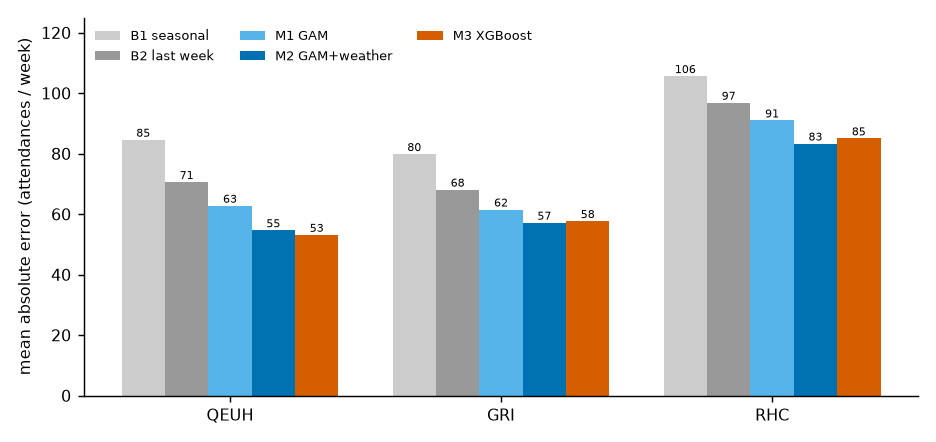
\includegraphics[width=0.9\textwidth]{../analysis/figures/fig_mae.png}
\caption{MAE by model and hospital, one week ahead.}
\end{figure}

\subsection{Which environmental factors matter}
Adding groups of weather variables to M1 one at a time showed that temperature carries the gain. Temperature alone gave MAE 54.9 (QEUH) and 57.7 (GRI), against 54.7 and 57.2 for all weather combined. Air quality alone (62.2 and 61.6) and humidity and rain alone (62.8 and 61.6) gave no improvement over M1 (all $p>0.4$ at the adult hospitals). A placebo model that was given the weather of the same week one year earlier lost the gain (QEUH 61.8, GRI 61.9), so the improvement is not a seasonal effect but depends on the temperature of the week itself.

The fitted GAM uses both this week's and last week's temperature, and the association is predictive, not causal. Moving only this week's temperature from the 5th to the 95th percentile (2.1 to 16.0\,$^\circ$C) with last week's temperature at its average was associated with about 150 more attendances at QEUH (8.1\% of the mean), 132 at GRI (8.0\%) and 153 at RHC (11.5\%). When last week's temperature moved with it, the association shrank to 38 at QEUH (2.0\%), 23 at GRI (1.4\%) and $-28$ at RHC. The signal is therefore mainly the week-to-week change in temperature: about 9.6 more attendances at QEUH and 9.8 at GRI for each degree a week is warmer than the previous one (about 0.5\% of weekly attendance). Weekly mean temperature in the test period stayed below 18\,$^\circ$C, so this says nothing about heatwaves.

\begin{figure}[h!]
\centering
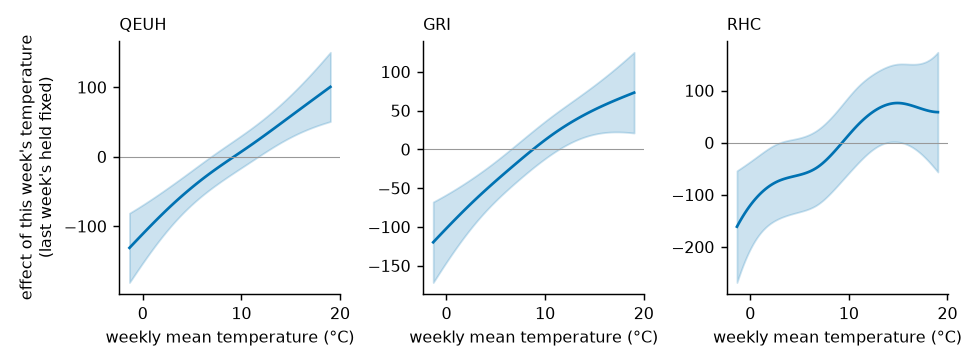
\includegraphics[width=0.9\textwidth]{../analysis/figures/fig_temperature_effect.png}
\caption{Association of this week's mean temperature with attendance (95\% band), with last week's temperature held fixed.}
\end{figure}

\subsection{Robustness}
Excluding flagged weeks from the training data did not change the one-week-ahead conclusions (QEUH: M2 52.3 against M1 60.6; GRI: 56.3 against 60.5; RHC: 77.7 against 86.8); the test weeks contain no flagged week. At two and four weeks ahead M2 beat M1 at QEUH (Holm $p=0.002$ at both horizons) but not at GRI or RHC, and the four-week result at QEUH is not significant when flagged weeks are excluded (Holm $p=0.236$). These longer horizons are not realistic forecasts, because the model sees the observed weather of a week that could not be known so far ahead; they are upper bounds.

\subsection{Real forecast weather}\label{sec:res-fw}
Archived ECMWF forecasts are available only from March 2024, so this experiment uses 135 of the 146 test weeks. Models trained on reanalysis weather were tested on the forecast issued the Sunday before each week (weekly mean-temperature error against reanalysis: RMSE 0.68\,$^\circ$C, bias $+0.30$\,$^\circ$C). At QEUH the gain was kept in full (MAE 54.4 against 62.4 for M1, Holm $p<0.001$). At GRI only part of it was kept: 59.9 against 62.9, not significant ($p=0.252$), and significantly worse than with observed weather (Holm $p=0.026$); its skill against last week was 13.2\%, below the 15\% target set in the proposal. The temperature-only model (M2t) was as good as M2 with forecast weather (54.3, 60.0 and 83.3 at QEUH, GRI and RHC), and is the model used in the prototype.

\subsection{Alerts}
A high-pressure week was defined as one above the 90th percentile of the previous 52 weeks. The first evaluation was for M2 with observed weather; the temperature-only model used in the prototype, real forecast weather and a ``medium'' tier (above the 75th percentile) were evaluated afterwards from the same forecasts (Section~5b of the results file). At QEUH, M2 raised 11 alerts for 21 high weeks, with precision 0.64 (95\% interval 0.35 to 0.85), recall 0.33 (0.17 to 0.55) and 0.12 false alarms per month; last-week persistence had recall 0.43 but precision 0.41 and 0.39 false alarms per month. At GRI, M2 had precision 0.55 and recall 0.44. At RHC (exploratory) M2 had precision 0.73 and recall 0.55 against 0.60 and 0.60 for persistence. At the two adult hospitals no model identified most high-pressure weeks, and the intervals are wide because there are few alerts. With the temperature-only model on real forecasts, the QEUH alert had precision 0.62 and recall 0.38 against a base rate of 15.6\%, with 0.16 false alarms per month, against 0.42 for last-week persistence at similar recall; at GRI the intervals overlapped with persistence, so no advantage was shown. The medium tier was only modestly informative (QEUH precision 0.60 against a base rate of 37.0\%) and the prototype keeps it as watch-only.

\section{Discussion}
The results support the central claim that weekly A\&E attendance in Glasgow can be forecast more accurately than by repeating last week, and that temperature explains part of that gain at the largest adult hospital. The pattern is consistent with the positive association between temperature and A\&E attendances reported for London \parencite{corcuerahotz2020}, although that study used daily data and a different method. It differs from the finding that temperature gave no better forecasts than calendar variables in S\~ao Paulo \parencite{marcilio2013}; the settings, the time scale (daily against weekly) and the three-month test window of that study are possible reasons, but this project cannot tell. The finding that a GAM matched XGBoost agrees with the observation that linear models are often as good as tree ensembles \parencite{vollmer2021}.

The gains are real but modest in absolute terms: about 8 attendances a week at QEUH on a weekly mean of about 1,850. The evidence for weather is strongest at QEUH, weaker at GRI (not significant under Holm correction, and partly lost with real forecasts), and exploratory at RHC. Evaluation choices matter: a rolling-origin test against a persistence baseline \parencite{garciacrespi2026} was used here, and the calendar and autoregressive terms accounted for about half of the improvement over last week, which a comparison with a seasonal baseline alone would have hidden.

\textbf{Limitations.} The test covers one city and 146 weeks; one weather grid cell stands for all three hospitals; the counts are all-cause and the data hold no infection information, so warm-week effects may partly reflect other seasonal factors. The result is predictive, not causal. The evaluation is not a real-time one: it assumes last week's attendance is known on the Sunday night, although the data are published with a delay, and it uses final, not first-release, figures. The model specifications were set before the experiments were run, to the author's knowledge, but the ablation, the placebo and the choice of the temperature-only model for the prototype came afterwards. Holm correction covers two hospitals per comparison, not the roughly 540 tests run, and the Diebold--Mariano test is approximate for nested models. Weather is reanalysis, not station data, and air quality is modelled. Hot-day thresholds were set from percentiles of pre-2024 temperatures, not from the GAM curves as planned in the interim report.

\section{Conclusion}
Weekly A\&E attendance at QEUH and GRI can be forecast better than by last week's value or the same week last year (reductions in MAE of 22.5\% and 16.0\% against last week). Temperature adds significant accuracy at QEUH (12.9\%) and inconclusively at GRI (7.1\%, $p=0.054$), mainly through the week-to-week change in temperature; air quality, humidity and rain add nothing. With real forecasts the gain holds at QEUH and weakens at GRI. The prototype turns the model into a one-week forecast with a risk class, an explanation of its drivers and a human approval step, but its alerts miss most high-pressure weeks at the adult hospitals and should be treated as a prompt for review. Future work includes infection data, station weather, school terms and local holidays, and testing across other Scottish boards.
 inside the final report's main.tex.
% Every number comes from ../analysis/results/results_tables.md (checked by ../analysis/check_results.py).
% The student must rewrite this in their own words (university AI-writing policy) and understand every sentence.
% Needs \usepackage{booktabs} for the tables and the figures in ../analysis/figures/.
% The word limit for the final report is not known yet: check the final-report template before keeping all of this.

\section{Results}\label{sec:results}

\subsection{Set-up}
Models were evaluated by rolling-origin testing on 146 weeks (7 January 2024 to 18 October 2026), with an expanding training window and a weekly re-fit. Hyper-parameters were re-tuned every 26 weeks using only the data available at that origin. Differences in mean absolute error (MAE) were tested with the Diebold--Mariano test \parencite{diebold1995} at the 5\% level, with the Holm correction across QEUH and GRI; RHC is exploratory and uncorrected. The primary comparisons, named before the tables were read, are M2 against M1 (H$_1$) and M2 against B2 (H$_2$) at QEUH and GRI, one week ahead; everything else is secondary or exploratory. The weather used in the main experiment is the observed (reanalysis) weather of the target week, so the main results show what weather can add when it is known (a nowcast); Section~\ref{sec:res-fw} uses real archived forecasts. Because M2 contains M1, the Diebold--Mariano asymptotics are approximate and borderline results are not decisive.

\subsection{Baselines and models, one week ahead}
\begin{table}[h!]
\centering\small
\begin{tabular}{lccc}
\hline
MAE (attendances per week) & QEUH & GRI & RHC \\
\hline
B1 seasonal naive & 84.6 & 79.8 & 105.6 \\
B2 last week & 70.6 & 68.1 & 96.8 \\
M1 GAM, no weather & 62.8 & 61.5 & 91.0 \\
M2 GAM with weather & 54.7 & 57.2 & 83.3 \\
M3 XGBoost, all features & 53.1 & 57.7 & 85.0 \\
M3a XGBoost, no weather & 56.7 & 60.2 & 86.7 \\
\hline
\end{tabular}
\caption{One-week-ahead errors on the 146 test weeks.}
\label{table:res-main}
\end{table}

\textbf{H$_2$ (beats the baselines, with observed weather).} M2 had a lower MAE than last week's attendance by 22.5\% at QEUH and 16.0\% at GRI (all Holm-adjusted $p<0.001$), and by 13.9\% at RHC. It also beat the seasonal baseline at every hospital.

\textbf{H$_1$ (weather adds value).} At QEUH, M2 reduced MAE by 12.9\% compared with the same model without weather (62.8 to 54.7; Holm-adjusted $p<0.001$). At GRI the reduction was 7.1\% (61.5 to 57.2) but the difference was not significant at the 5\% level ($p=0.054$), so the null hypothesis is not rejected there; with a Newey--West variance the same comparison gave $p=0.024$ and $0.015$ (3 and 8 lags), so GRI is best described as inconclusive. At RHC (exploratory) the difference was significant ($p=0.002$, uncorrected). About half of M2's improvement over last week at QEUH comes from the calendar and autoregressive terms: M1 alone has 11.1\% skill against last week, M2 has 22.5\%.

At one week ahead XGBoost did not improve on the GAM: M3 and M2 did not differ significantly (Holm $p=0.935$ at both adult hospitals). At two weeks ahead M3 was lower than M2 at QEUH (54.1 against 59.6) but not significantly so after correction (Holm $p=0.059$).

\begin{figure}[h!]
\centering
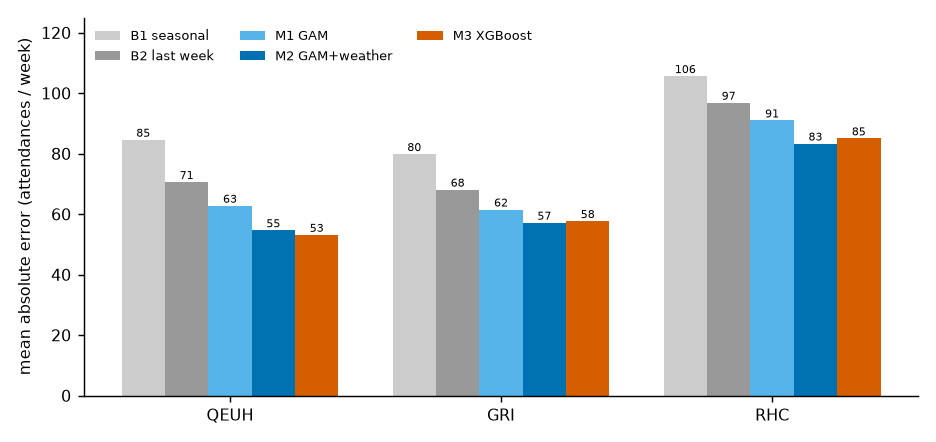
\includegraphics[width=0.9\textwidth]{../analysis/figures/fig_mae.png}
\caption{MAE by model and hospital, one week ahead.}
\end{figure}

\subsection{Which environmental factors matter}
Adding groups of weather variables to M1 one at a time showed that temperature carries the gain. Temperature alone gave MAE 54.9 (QEUH) and 57.7 (GRI), against 54.7 and 57.2 for all weather combined. Air quality alone (62.2 and 61.6) and humidity and rain alone (62.8 and 61.6) gave no improvement over M1 (all $p>0.4$ at the adult hospitals). A placebo model that was given the weather of the same week one year earlier lost the gain (QEUH 61.8, GRI 61.9), so the improvement is not a seasonal effect but depends on the temperature of the week itself.

The fitted GAM uses both this week's and last week's temperature, and the association is predictive, not causal. Moving only this week's temperature from the 5th to the 95th percentile (2.1 to 16.0\,$^\circ$C) with last week's temperature at its average was associated with about 150 more attendances at QEUH (8.1\% of the mean), 132 at GRI (8.0\%) and 153 at RHC (11.5\%). When last week's temperature moved with it, the association shrank to 38 at QEUH (2.0\%), 23 at GRI (1.4\%) and $-28$ at RHC. The signal is therefore mainly the week-to-week change in temperature: about 9.6 more attendances at QEUH and 9.8 at GRI for each degree a week is warmer than the previous one (about 0.5\% of weekly attendance). Weekly mean temperature in the test period stayed below 18\,$^\circ$C, so this says nothing about heatwaves.

\begin{figure}[h!]
\centering
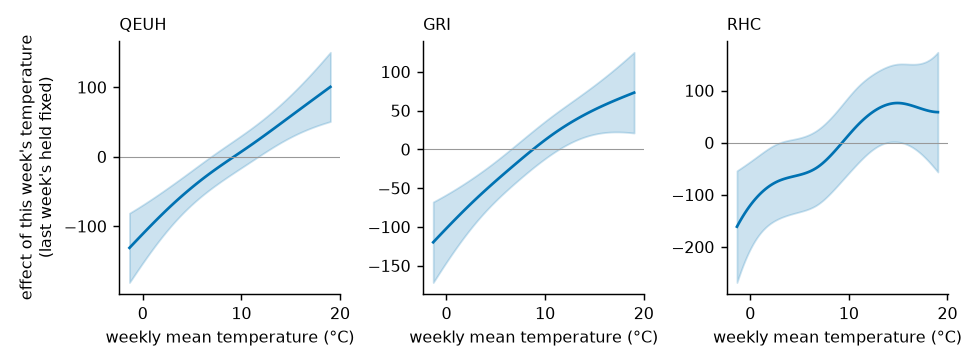
\includegraphics[width=0.9\textwidth]{../analysis/figures/fig_temperature_effect.png}
\caption{Association of this week's mean temperature with attendance (95\% band), with last week's temperature held fixed.}
\end{figure}

\subsection{Robustness}
Excluding flagged weeks from the training data did not change the one-week-ahead conclusions (QEUH: M2 52.3 against M1 60.6; GRI: 56.3 against 60.5; RHC: 77.7 against 86.8); the test weeks contain no flagged week. At two and four weeks ahead M2 beat M1 at QEUH (Holm $p=0.002$ at both horizons) but not at GRI or RHC, and the four-week result at QEUH is not significant when flagged weeks are excluded (Holm $p=0.236$). These longer horizons are not realistic forecasts, because the model sees the observed weather of a week that could not be known so far ahead; they are upper bounds.

\subsection{Real forecast weather}\label{sec:res-fw}
Archived ECMWF forecasts are available only from March 2024, so this experiment uses 135 of the 146 test weeks. Models trained on reanalysis weather were tested on the forecast issued the Sunday before each week (weekly mean-temperature error against reanalysis: RMSE 0.68\,$^\circ$C, bias $+0.30$\,$^\circ$C). At QEUH the gain was kept in full (MAE 54.4 against 62.4 for M1, Holm $p<0.001$). At GRI only part of it was kept: 59.9 against 62.9, not significant ($p=0.252$), and significantly worse than with observed weather (Holm $p=0.026$); its skill against last week was 13.2\%, below the 15\% target set in the proposal. The temperature-only model (M2t) was as good as M2 with forecast weather (54.3, 60.0 and 83.3 at QEUH, GRI and RHC), and is the model used in the prototype.

\subsection{Alerts}
A high-pressure week was defined as one above the 90th percentile of the previous 52 weeks. The first evaluation was for M2 with observed weather; the temperature-only model used in the prototype, real forecast weather and a ``medium'' tier (above the 75th percentile) were evaluated afterwards from the same forecasts (Section~5b of the results file). At QEUH, M2 raised 11 alerts for 21 high weeks, with precision 0.64 (95\% interval 0.35 to 0.85), recall 0.33 (0.17 to 0.55) and 0.12 false alarms per month; last-week persistence had recall 0.43 but precision 0.41 and 0.39 false alarms per month. At GRI, M2 had precision 0.55 and recall 0.44. At RHC (exploratory) M2 had precision 0.73 and recall 0.55 against 0.60 and 0.60 for persistence. At the two adult hospitals no model identified most high-pressure weeks, and the intervals are wide because there are few alerts. With the temperature-only model on real forecasts, the QEUH alert had precision 0.62 and recall 0.38 against a base rate of 15.6\%, with 0.16 false alarms per month, against 0.42 for last-week persistence at similar recall; at GRI the intervals overlapped with persistence, so no advantage was shown. The medium tier was only modestly informative (QEUH precision 0.60 against a base rate of 37.0\%) and the prototype keeps it as watch-only.

\section{Discussion}
The results support the central claim that weekly A\&E attendance in Glasgow can be forecast more accurately than by repeating last week, and that temperature explains part of that gain at the largest adult hospital. The pattern is consistent with the positive association between temperature and A\&E attendances reported for London \parencite{corcuerahotz2020}, although that study used daily data and a different method. It differs from the finding that temperature gave no better forecasts than calendar variables in S\~ao Paulo \parencite{marcilio2013}; the settings, the time scale (daily against weekly) and the three-month test window of that study are possible reasons, but this project cannot tell. The finding that a GAM matched XGBoost agrees with the observation that linear models are often as good as tree ensembles \parencite{vollmer2021}.

The gains are real but modest in absolute terms: about 8 attendances a week at QEUH on a weekly mean of about 1,850. The evidence for weather is strongest at QEUH, weaker at GRI (not significant under Holm correction, and partly lost with real forecasts), and exploratory at RHC. Evaluation choices matter: a rolling-origin test against a persistence baseline \parencite{garciacrespi2026} was used here, and the calendar and autoregressive terms accounted for about half of the improvement over last week, which a comparison with a seasonal baseline alone would have hidden.

\textbf{Limitations.} The test covers one city and 146 weeks; one weather grid cell stands for all three hospitals; the counts are all-cause and the data hold no infection information, so warm-week effects may partly reflect other seasonal factors. The result is predictive, not causal. The evaluation is not a real-time one: it assumes last week's attendance is known on the Sunday night, although the data are published with a delay, and it uses final, not first-release, figures. The model specifications were set before the experiments were run, to the author's knowledge, but the ablation, the placebo and the choice of the temperature-only model for the prototype came afterwards. Holm correction covers two hospitals per comparison, not the roughly 540 tests run, and the Diebold--Mariano test is approximate for nested models. Weather is reanalysis, not station data, and air quality is modelled. Hot-day thresholds were set from percentiles of pre-2024 temperatures, not from the GAM curves as planned in the interim report.

\section{Conclusion}
Weekly A\&E attendance at QEUH and GRI can be forecast better than by last week's value or the same week last year (reductions in MAE of 22.5\% and 16.0\% against last week). Temperature adds significant accuracy at QEUH (12.9\%) and inconclusively at GRI (7.1\%, $p=0.054$), mainly through the week-to-week change in temperature; air quality, humidity and rain add nothing. With real forecasts the gain holds at QEUH and weakens at GRI. The prototype turns the model into a one-week forecast with a risk class, an explanation of its drivers and a human approval step, but its alerts miss most high-pressure weeks at the adult hospitals and should be treated as a prompt for review. Future work includes infection data, station weather, school terms and local holidays, and testing across other Scottish boards.
 inside the final report's main.tex.
% Every number comes from ../analysis/results/results_tables.md (checked by ../analysis/check_results.py).
% The student must rewrite this in their own words (university AI-writing policy) and understand every sentence.
% Needs \usepackage{booktabs} for the tables and the figures in ../analysis/figures/.
% The word limit for the final report is not known yet: check the final-report template before keeping all of this.

\section{Results}\label{sec:results}

\subsection{Set-up}
Models were evaluated by rolling-origin testing on 146 weeks (7 January 2024 to 18 October 2026), with an expanding training window and a weekly re-fit. Hyper-parameters were re-tuned every 26 weeks using only the data available at that origin. Differences in mean absolute error (MAE) were tested with the Diebold--Mariano test \parencite{diebold1995} at the 5\% level, with the Holm correction across QEUH and GRI; RHC is exploratory and uncorrected. The primary comparisons, named before the tables were read, are M2 against M1 (H$_1$) and M2 against B2 (H$_2$) at QEUH and GRI, one week ahead; everything else is secondary or exploratory. The weather used in the main experiment is the observed (reanalysis) weather of the target week, so the main results show what weather can add when it is known (a nowcast); Section~\ref{sec:res-fw} uses real archived forecasts. Because M2 contains M1, the Diebold--Mariano asymptotics are approximate and borderline results are not decisive.

\subsection{Baselines and models, one week ahead}
\begin{table}[h!]
\centering\small
\begin{tabular}{lccc}
\hline
MAE (attendances per week) & QEUH & GRI & RHC \\
\hline
B1 seasonal naive & 84.6 & 79.8 & 105.6 \\
B2 last week & 70.6 & 68.1 & 96.8 \\
M1 GAM, no weather & 62.8 & 61.5 & 91.0 \\
M2 GAM with weather & 54.7 & 57.2 & 83.3 \\
M3 XGBoost, all features & 53.1 & 57.7 & 85.0 \\
M3a XGBoost, no weather & 56.7 & 60.2 & 86.7 \\
\hline
\end{tabular}
\caption{One-week-ahead errors on the 146 test weeks.}
\label{table:res-main}
\end{table}

\textbf{H$_2$ (beats the baselines, with observed weather).} M2 had a lower MAE than last week's attendance by 22.5\% at QEUH and 16.0\% at GRI (all Holm-adjusted $p<0.001$), and by 13.9\% at RHC. It also beat the seasonal baseline at every hospital.

\textbf{H$_1$ (weather adds value).} At QEUH, M2 reduced MAE by 12.9\% compared with the same model without weather (62.8 to 54.7; Holm-adjusted $p<0.001$). At GRI the reduction was 7.1\% (61.5 to 57.2) but the difference was not significant at the 5\% level ($p=0.054$), so the null hypothesis is not rejected there; with a Newey--West variance the same comparison gave $p=0.024$ and $0.015$ (3 and 8 lags), so GRI is best described as inconclusive. At RHC (exploratory) the difference was significant ($p=0.002$, uncorrected). About half of M2's improvement over last week at QEUH comes from the calendar and autoregressive terms: M1 alone has 11.1\% skill against last week, M2 has 22.5\%.

At one week ahead XGBoost did not improve on the GAM: M3 and M2 did not differ significantly (Holm $p=0.935$ at both adult hospitals). At two weeks ahead M3 was lower than M2 at QEUH (54.1 against 59.6) but not significantly so after correction (Holm $p=0.059$).

\begin{figure}[h!]
\centering
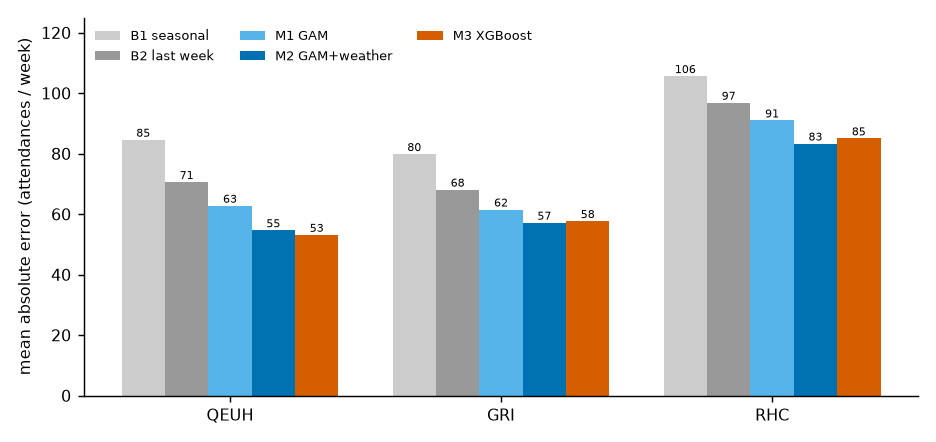
\includegraphics[width=0.9\textwidth]{../analysis/figures/fig_mae.png}
\caption{MAE by model and hospital, one week ahead.}
\end{figure}

\subsection{Which environmental factors matter}
Adding groups of weather variables to M1 one at a time showed that temperature carries the gain. Temperature alone gave MAE 54.9 (QEUH) and 57.7 (GRI), against 54.7 and 57.2 for all weather combined. Air quality alone (62.2 and 61.6) and humidity and rain alone (62.8 and 61.6) gave no improvement over M1 (all $p>0.4$ at the adult hospitals). A placebo model that was given the weather of the same week one year earlier lost the gain (QEUH 61.8, GRI 61.9), so the improvement is not a seasonal effect but depends on the temperature of the week itself.

The fitted GAM uses both this week's and last week's temperature, and the association is predictive, not causal. Moving only this week's temperature from the 5th to the 95th percentile (2.1 to 16.0\,$^\circ$C) with last week's temperature at its average was associated with about 150 more attendances at QEUH (8.1\% of the mean), 132 at GRI (8.0\%) and 153 at RHC (11.5\%). When last week's temperature moved with it, the association shrank to 38 at QEUH (2.0\%), 23 at GRI (1.4\%) and $-28$ at RHC. The signal is therefore mainly the week-to-week change in temperature: about 9.6 more attendances at QEUH and 9.8 at GRI for each degree a week is warmer than the previous one (about 0.5\% of weekly attendance). Weekly mean temperature in the test period stayed below 18\,$^\circ$C, so this says nothing about heatwaves.

\begin{figure}[h!]
\centering
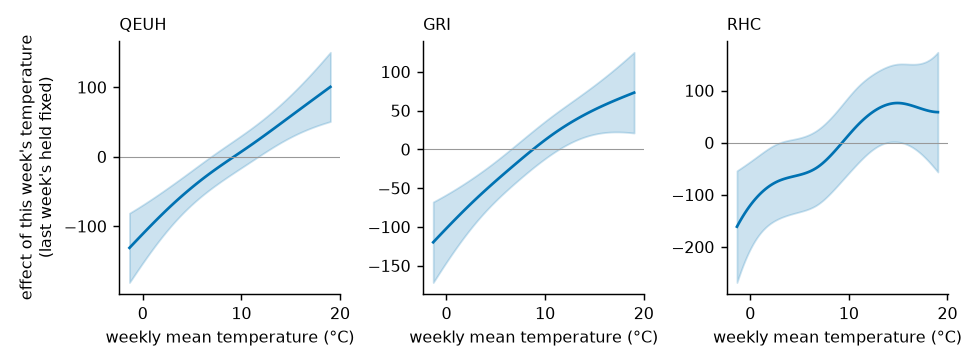
\includegraphics[width=0.9\textwidth]{../analysis/figures/fig_temperature_effect.png}
\caption{Association of this week's mean temperature with attendance (95\% band), with last week's temperature held fixed.}
\end{figure}

\subsection{Robustness}
Excluding flagged weeks from the training data did not change the one-week-ahead conclusions (QEUH: M2 52.3 against M1 60.6; GRI: 56.3 against 60.5; RHC: 77.7 against 86.8); the test weeks contain no flagged week. At two and four weeks ahead M2 beat M1 at QEUH (Holm $p=0.002$ at both horizons) but not at GRI or RHC, and the four-week result at QEUH is not significant when flagged weeks are excluded (Holm $p=0.236$). These longer horizons are not realistic forecasts, because the model sees the observed weather of a week that could not be known so far ahead; they are upper bounds.

\subsection{Real forecast weather}\label{sec:res-fw}
Archived ECMWF forecasts are available only from March 2024, so this experiment uses 135 of the 146 test weeks. Models trained on reanalysis weather were tested on the forecast issued the Sunday before each week (weekly mean-temperature error against reanalysis: RMSE 0.68\,$^\circ$C, bias $+0.30$\,$^\circ$C). At QEUH the gain was kept in full (MAE 54.4 against 62.4 for M1, Holm $p<0.001$). At GRI only part of it was kept: 59.9 against 62.9, not significant ($p=0.252$), and significantly worse than with observed weather (Holm $p=0.026$); its skill against last week was 13.2\%, below the 15\% target set in the proposal. The temperature-only model (M2t) was as good as M2 with forecast weather (54.3, 60.0 and 83.3 at QEUH, GRI and RHC), and is the model used in the prototype.

\subsection{Alerts}
A high-pressure week was defined as one above the 90th percentile of the previous 52 weeks. The first evaluation was for M2 with observed weather; the temperature-only model used in the prototype, real forecast weather and a ``medium'' tier (above the 75th percentile) were evaluated afterwards from the same forecasts (Section~5b of the results file). At QEUH, M2 raised 11 alerts for 21 high weeks, with precision 0.64 (95\% interval 0.35 to 0.85), recall 0.33 (0.17 to 0.55) and 0.12 false alarms per month; last-week persistence had recall 0.43 but precision 0.41 and 0.39 false alarms per month. At GRI, M2 had precision 0.55 and recall 0.44. At RHC (exploratory) M2 had precision 0.73 and recall 0.55 against 0.60 and 0.60 for persistence. At the two adult hospitals no model identified most high-pressure weeks, and the intervals are wide because there are few alerts. With the temperature-only model on real forecasts, the QEUH alert had precision 0.62 and recall 0.38 against a base rate of 15.6\%, with 0.16 false alarms per month, against 0.42 for last-week persistence at similar recall; at GRI the intervals overlapped with persistence, so no advantage was shown. The medium tier was only modestly informative (QEUH precision 0.60 against a base rate of 37.0\%) and the prototype keeps it as watch-only.

\section{Discussion}
The results support the central claim that weekly A\&E attendance in Glasgow can be forecast more accurately than by repeating last week, and that temperature explains part of that gain at the largest adult hospital. The pattern is consistent with the positive association between temperature and A\&E attendances reported for London \parencite{corcuerahotz2020}, although that study used daily data and a different method. It differs from the finding that temperature gave no better forecasts than calendar variables in S\~ao Paulo \parencite{marcilio2013}; the settings, the time scale (daily against weekly) and the three-month test window of that study are possible reasons, but this project cannot tell. The finding that a GAM matched XGBoost agrees with the observation that linear models are often as good as tree ensembles \parencite{vollmer2021}.

The gains are real but modest in absolute terms: about 8 attendances a week at QEUH on a weekly mean of about 1,850. The evidence for weather is strongest at QEUH, weaker at GRI (not significant under Holm correction, and partly lost with real forecasts), and exploratory at RHC. Evaluation choices matter: a rolling-origin test against a persistence baseline \parencite{garciacrespi2026} was used here, and the calendar and autoregressive terms accounted for about half of the improvement over last week, which a comparison with a seasonal baseline alone would have hidden.

\textbf{Limitations.} The test covers one city and 146 weeks; one weather grid cell stands for all three hospitals; the counts are all-cause and the data hold no infection information, so warm-week effects may partly reflect other seasonal factors. The result is predictive, not causal. The evaluation is not a real-time one: it assumes last week's attendance is known on the Sunday night, although the data are published with a delay, and it uses final, not first-release, figures. The model specifications were set before the experiments were run, to the author's knowledge, but the ablation, the placebo and the choice of the temperature-only model for the prototype came afterwards. Holm correction covers two hospitals per comparison, not the roughly 540 tests run, and the Diebold--Mariano test is approximate for nested models. Weather is reanalysis, not station data, and air quality is modelled. Hot-day thresholds were set from percentiles of pre-2024 temperatures, not from the GAM curves as planned in the interim report.

\section{Conclusion}
Weekly A\&E attendance at QEUH and GRI can be forecast better than by last week's value or the same week last year (reductions in MAE of 22.5\% and 16.0\% against last week). Temperature adds significant accuracy at QEUH (12.9\%) and inconclusively at GRI (7.1\%, $p=0.054$), mainly through the week-to-week change in temperature; air quality, humidity and rain add nothing. With real forecasts the gain holds at QEUH and weakens at GRI. The prototype turns the model into a one-week forecast with a risk class, an explanation of its drivers and a human approval step, but its alerts miss most high-pressure weeks at the adult hospitals and should be treated as a prompt for review. Future work includes infection data, station weather, school terms and local holidays, and testing across other Scottish boards.
